\documentclass{standalone}
\usepackage{tikz}
\usetikzlibrary{patterns, positioning}

\begin{document}
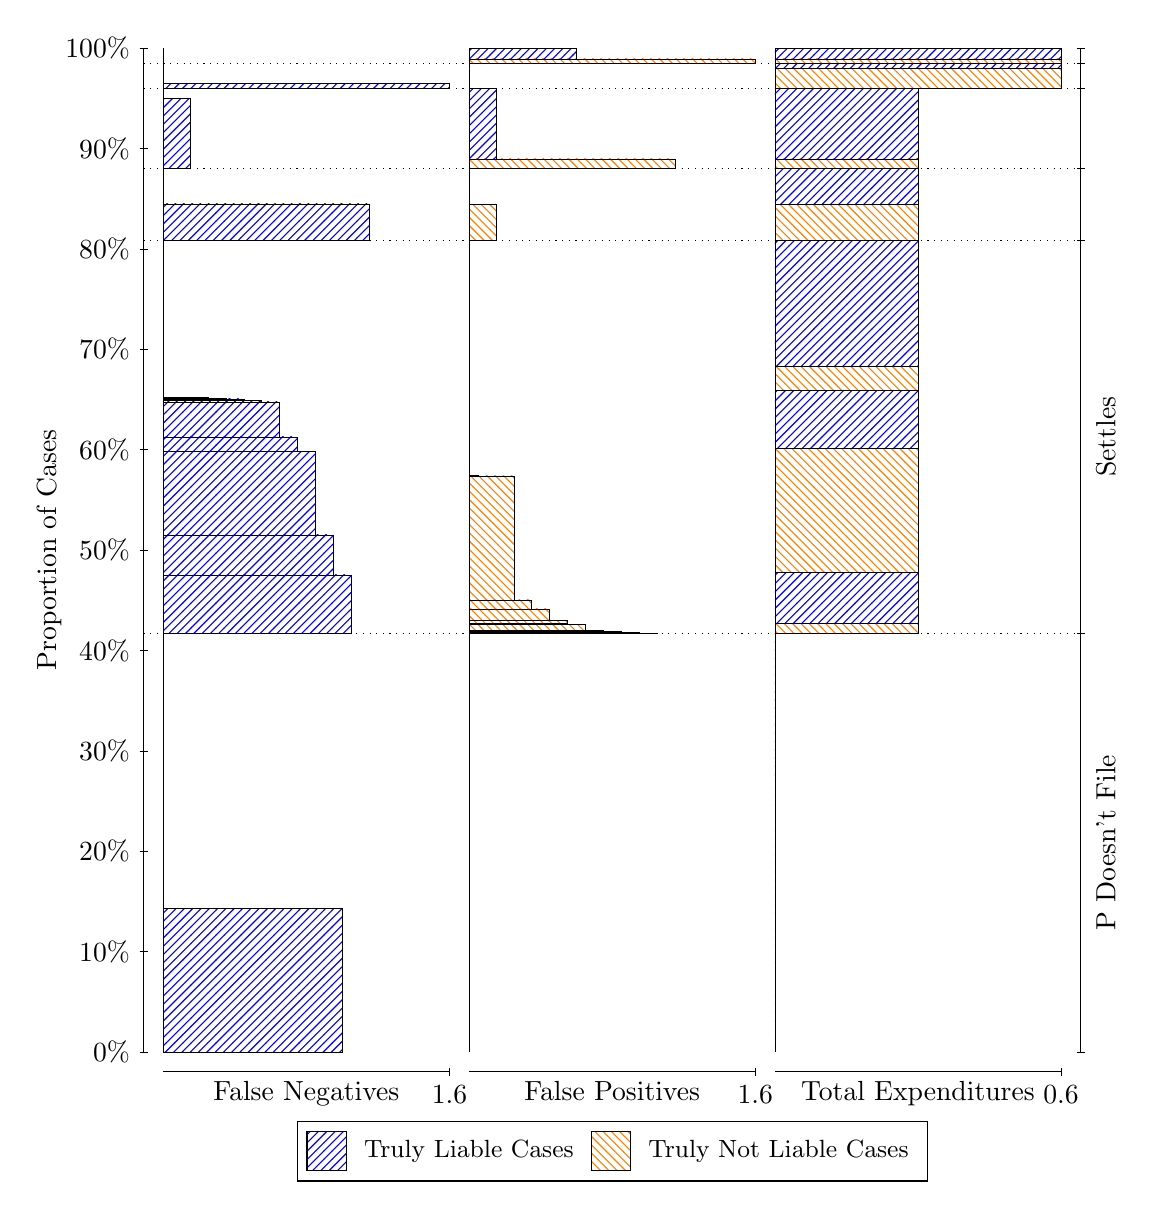
\begin{tikzpicture}
\draw[black, very thin] (1.5,1.75) -- (1.5,14.5);
\node[rotate=90, anchor=center] at (0.3, 8.125) {Proportion of Cases};
\draw[black, very thin] (1.45,1.75) -- (1.55,1.75);
\node[anchor=east] at (1.45, 1.75) {0\%};
\draw[black, very thin] (1.45,3.025) -- (1.55,3.025);
\node[anchor=east] at (1.45, 3.025) {10\%};
\draw[black, very thin] (1.45,4.3) -- (1.55,4.3);
\node[anchor=east] at (1.45, 4.3) {20\%};
\draw[black, very thin] (1.45,5.575) -- (1.55,5.575);
\node[anchor=east] at (1.45, 5.575) {30\%};
\draw[black, very thin] (1.45,6.85) -- (1.55,6.85);
\node[anchor=east] at (1.45, 6.85) {40\%};
\draw[black, very thin] (1.45,8.125) -- (1.55,8.125);
\node[anchor=east] at (1.45, 8.125) {50\%};
\draw[black, very thin] (1.45,9.4) -- (1.55,9.4);
\node[anchor=east] at (1.45, 9.4) {60\%};
\draw[black, very thin] (1.45,10.675) -- (1.55,10.675);
\node[anchor=east] at (1.45, 10.675) {70\%};
\draw[black, very thin] (1.45,11.95) -- (1.55,11.95);
\node[anchor=east] at (1.45, 11.95) {80\%};
\draw[black, very thin] (1.45,13.225) -- (1.55,13.225);
\node[anchor=east] at (1.45, 13.225) {90\%};
\draw[black, very thin] (1.45,14.5) -- (1.55,14.5);
\node[anchor=east] at (1.45, 14.5) {100\%};

\draw[black, very thin] (13.4,1.75) -- (13.4,14.5);
\draw[black, very thin] (13.35,1.75) -- (13.45,1.75);
\node[anchor=west] at (13.35, 1.75) {};
\draw[black, very thin] (13.35,7.0661) -- (13.45,7.0661);
\node[anchor=west] at (13.35, 7.0661) {};
\draw[black, very thin] (13.35,12.061) -- (13.45,12.061);
\node[anchor=west] at (13.35, 12.061) {};
\draw[black, very thin] (13.35,12.971) -- (13.45,12.971);
\node[anchor=west] at (13.35, 12.971) {};
\draw[black, very thin] (13.35,13.985) -- (13.45,13.985);
\node[anchor=west] at (13.35, 13.985) {};
\draw[black, very thin] (13.35,14.308) -- (13.45,14.308);
\node[anchor=west] at (13.35, 14.308) {};
\draw[black, very thin] (13.35,14.5) -- (13.45,14.5);
\node[anchor=west] at (13.35, 14.5) {};

\draw[black, very thin, pattern color=blue, pattern=north east lines] (1.75,1.75) rectangle (4.0208,3.5751);
\draw[black, very thin, pattern color=orange, pattern=north west lines] (1.75,3.5751) rectangle (1.75,7.0661);
\draw[black, very thin, pattern color=blue, pattern=north east lines] (1.75,7.0661) rectangle (4.1344,7.8102);
\draw[black, very thin, pattern color=blue, pattern=north east lines] (1.75,7.8102) rectangle (3.9073,8.3177);
\draw[black, very thin, pattern color=blue, pattern=north east lines] (1.75,8.3177) rectangle (3.6802,9.3777);
\draw[black, very thin, pattern color=blue, pattern=north east lines] (1.75,9.3777) rectangle (3.4531,9.5629);
\draw[black, very thin, pattern color=blue, pattern=north east lines] (1.75,9.5629) rectangle (3.226,10.006);
\draw[black, very thin, pattern color=blue, pattern=north east lines] (1.75,10.006) rectangle (2.999,10.023);
\draw[black, very thin, pattern color=blue, pattern=north east lines] (1.75,10.023) rectangle (2.7719,10.043);
\draw[black, very thin, pattern color=blue, pattern=north east lines] (1.75,10.043) rectangle (2.5448,10.052);
\draw[black, very thin, pattern color=blue, pattern=north east lines] (1.75,10.052) rectangle (2.3177,10.06);
\draw[black, very thin, pattern color=orange, pattern=north west lines] (1.75,10.06) rectangle (1.75,12.061);
\draw[black, very thin, pattern color=blue, pattern=north east lines] (1.75,12.061) rectangle (4.3615,12.522);
\draw[black, very thin, pattern color=orange, pattern=north west lines] (1.75,12.522) rectangle (1.75,12.971);
\draw[black, very thin, pattern color=blue, pattern=north east lines] (1.75,12.971) rectangle (2.0906,13.863);
\draw[black, very thin, pattern color=orange, pattern=north west lines] (1.75,13.863) rectangle (1.75,13.985);
\draw[black, very thin, pattern color=blue, pattern=north east lines] (1.75,13.985) rectangle (5.3833,14.05);
\draw[black, very thin, pattern color=orange, pattern=north west lines] (1.75,14.05) rectangle (1.75,14.308);
\draw[black, very thin, pattern color=orange, pattern=north west lines] (1.75,14.308) rectangle (1.75,14.362);
\draw[black, very thin, pattern color=blue, pattern=north east lines] (1.75,14.362) rectangle (1.75,14.5);
\draw[black, very thin, pattern color=orange, pattern=north west lines] (5.6333,1.75) rectangle (5.6333,5.241);
\draw[black, very thin, pattern color=blue, pattern=north east lines] (5.6333,5.241) rectangle (5.6333,7.0661);
\draw[black, very thin, pattern color=orange, pattern=north west lines] (5.6333,7.0661) rectangle (8.0177,7.0707);
\draw[black, very thin, pattern color=orange, pattern=north west lines] (5.6333,7.0707) rectangle (7.7906,7.0763);
\draw[black, very thin, pattern color=orange, pattern=north west lines] (5.6333,7.0763) rectangle (7.5635,7.0891);
\draw[black, very thin, pattern color=orange, pattern=north west lines] (5.6333,7.0891) rectangle (7.3365,7.0998);
\draw[black, very thin, pattern color=orange, pattern=north west lines] (5.6333,7.0998) rectangle (7.1094,7.1781);
\draw[black, very thin, pattern color=orange, pattern=north west lines] (5.6333,7.1781) rectangle (6.8823,7.1954);
\draw[black, very thin, pattern color=orange, pattern=north west lines] (5.6333,7.1954) rectangle (6.8823,7.2273);
\draw[black, very thin, pattern color=orange, pattern=north west lines] (5.6333,7.2273) rectangle (6.6552,7.3765);
\draw[black, very thin, pattern color=orange, pattern=north west lines] (5.6333,7.3765) rectangle (6.4281,7.492);
\draw[black, very thin, pattern color=orange, pattern=north west lines] (5.6333,7.492) rectangle (6.201,9.0674);
\draw[black, very thin, pattern color=blue, pattern=north east lines] (5.6333,9.0674) rectangle (5.7469,9.0745);
\draw[black, very thin, pattern color=blue, pattern=north east lines] (5.6333,9.0745) rectangle (5.6333,12.061);
\draw[black, very thin, pattern color=orange, pattern=north west lines] (5.6333,12.061) rectangle (5.974,12.51);
\draw[black, very thin, pattern color=blue, pattern=north east lines] (5.6333,12.51) rectangle (5.6333,12.971);
\draw[black, very thin, pattern color=orange, pattern=north west lines] (5.6333,12.971) rectangle (8.2448,13.093);
\draw[black, very thin, pattern color=blue, pattern=north east lines] (5.6333,13.093) rectangle (5.974,13.985);
\draw[black, very thin, pattern color=orange, pattern=north west lines] (5.6333,13.985) rectangle (5.6333,14.243);
\draw[black, very thin, pattern color=blue, pattern=north east lines] (5.6333,14.243) rectangle (5.6333,14.308);
\draw[black, very thin, pattern color=orange, pattern=north west lines] (5.6333,14.308) rectangle (9.2667,14.362);
\draw[black, very thin, pattern color=blue, pattern=north east lines] (5.6333,14.362) rectangle (6.9958,14.5);
\draw[black, very thin, pattern color=orange, pattern=north west lines] (9.5167,1.75) rectangle (9.5167,5.241);
\draw[black, very thin, pattern color=blue, pattern=north east lines] (9.5167,5.241) rectangle (9.5167,7.0661);
\draw[black, very thin, pattern color=orange, pattern=north west lines] (9.5167,7.0661) rectangle (11.333,7.1954);
\draw[black, very thin, pattern color=blue, pattern=north east lines] (9.5167,7.1954) rectangle (11.333,7.8359);
\draw[black, very thin, pattern color=orange, pattern=north west lines] (9.5167,7.8359) rectangle (11.333,9.4113);
\draw[black, very thin, pattern color=blue, pattern=north east lines] (9.5167,9.4113) rectangle (11.333,10.155);
\draw[black, very thin, pattern color=orange, pattern=north west lines] (9.5167,10.155) rectangle (11.333,10.452);
\draw[black, very thin, pattern color=blue, pattern=north east lines] (9.5167,10.452) rectangle (11.333,12.061);
\draw[black, very thin, pattern color=orange, pattern=north west lines] (9.5167,12.061) rectangle (11.333,12.51);
\draw[black, very thin, pattern color=blue, pattern=north east lines] (9.5167,12.51) rectangle (11.333,12.971);
\draw[black, very thin, pattern color=orange, pattern=north west lines] (9.5167,12.971) rectangle (11.333,13.093);
\draw[black, very thin, pattern color=blue, pattern=north east lines] (9.5167,13.093) rectangle (11.333,13.985);
\draw[black, very thin, pattern color=orange, pattern=north west lines] (9.5167,13.985) rectangle (13.15,14.243);
\draw[black, very thin, pattern color=blue, pattern=north east lines] (9.5167,14.243) rectangle (13.15,14.308);
\draw[black, very thin, pattern color=orange, pattern=north west lines] (9.5167,14.308) rectangle (13.15,14.362);
\draw[black, very thin, pattern color=blue, pattern=north east lines] (9.5167,14.362) rectangle (13.15,14.5);
\draw[black, dotted] (1.5,7.0661) -- (13.4,7.0661);
\draw[black, dotted] (1.5,12.061) -- (13.4,12.061);
\draw[black, dotted] (1.5,12.971) -- (13.4,12.971);
\draw[black, dotted] (1.5,13.985) -- (13.4,13.985);
\draw[black, dotted] (1.5,14.308) -- (13.4,14.308);
\draw[black, very thin] (1.75,1.5) -- (5.3833,1.5);
\node[anchor=north] at (3.5667, 1.5) {False Negatives};
\draw[black, very thin] (5.3833,1.45) -- (5.3833,1.55);
\node[anchor=north] at (5.3833, 1.45) {1.6};

\draw[black, very thin] (5.6333,1.5) -- (9.2667,1.5);
\node[anchor=north] at (7.45, 1.5) {False Positives};
\draw[black, very thin] (9.2667,1.45) -- (9.2667,1.55);
\node[anchor=north] at (9.2667, 1.45) {1.6};

\draw[black, very thin] (9.5167,1.5) -- (13.15,1.5);
\node[anchor=north] at (11.333, 1.5) {Total Expenditures};
\draw[black, very thin] (13.15,1.45) -- (13.15,1.55);
\node[anchor=north] at (13.15, 1.45) {0.6};

\node[black, centered, rotate=90] at (13.72, 4.408) {P Doesn't File};
\node[black, centered, rotate=90] at (13.72, 9.5635) {Settles};





\draw (7.449999999999999,1.5) node[draw=none] (baseCoordinate) {};
\begin{scope}[align=center]
        \matrix[scale=0.5, draw=black, below=0.5cm of baseCoordinate, nodes={draw}, column sep=0.1cm]{
            \node[rectangle, draw, minimum width=0.5cm, minimum height=0.5cm, pattern=north east lines, pattern color=blue] {}; &
            \node[draw=none, font=\small] (B) {Truly Liable Cases}; &
            \node[rectangle, draw, minimum width=0.5cm, minimum height=0.5cm, pattern=north west lines, pattern color=orange] {}; &
            \node[draw=none, font=\small] (B) {Truly Not Liable Cases}; \\
            };
\end{scope}

\end{tikzpicture}
\end{document}